\documentclass[aspectratio=169]{beamer}
\usetheme{Madrid}
\usecolortheme{default}
\usepackage{graphicx}
\usepackage{booktabs}
\graphicspath{{figures/}}

\title[0D aortic banding]{A 0D pulsatile model of aortic-arch banding}
\subtitle{Reproducing carotid pulsatility redistribution (Eberth et al., 2009)}
\author{svZeroDSolver}
\date{\today}

\begin{document}

\begin{frame}\titlepage\end{frame}

% ---------------------------------------------------------------
\begin{frame}{The problem}
\textbf{Eberth et al. (2009):} a stiff band on the mouse aortic arch, placed
\emph{between} the two carotid takeoffs, creates paired carotids with
\alert{similar mean pressure \& flow but very different pulsatility}.
\begin{itemize}
  \item \textbf{RCCA-B} (right) — \emph{upstream} of the band: sees the full pulse
        + reflections $\Rightarrow$ pulsatility index rises (PI $\approx 3.11$).
  \item \textbf{LCCA-B} (left) — \emph{downstream}: the resistive--inertial band
        damps the pulse (PI $\approx 1.65$); baseline CCA $\approx 1.16$.
\end{itemize}
\vspace{1em}
\textbf{Goal:} a reduced-order (0D) lumped model that reproduces this
redistribution with the band as the only structural change --- and that maps to
the wall growth \& remodeling Eberth measured.
\end{frame}

% ---------------------------------------------------------------
\begin{frame}{The 0D model}
\small
Heart $\to$ aortic valve $\to$ ascending aorta $\to$ \textbf{node A} $\to$
band $\Delta P(Q)$ $\to$ \textbf{node B} $\to$ descending aorta; a carotid RCR
bed hangs off each node.
\begin{columns}[T]
\begin{column}{0.5\textwidth}
\begin{itemize}
  \item Vessels: RCL \texttt{BloodVessel} blocks
  \item Band: nonlinear \emph{Young--Tsai} stenosis \\
        $\Delta P=(R+S|Q|)Q + L\,\dot Q$
  \item Terminal beds: 3-element RCR windkessels
  \item Valve: \texttt{ValveTanh} diode
\end{itemize}
\end{column}
\begin{column}{0.5\textwidth}
\begin{itemize}
  \item Parameters from mouse literature \\ (geometry, blood, wall stiffness $E$)
  \item Every parameter tagged \\ \textsc{fixed} / \textsc{derived} / \textsc{calibrate}
  \item Only the band \texttt{stenosis\_coefficient} is calibrated
        (to the Table-1 PI ratio)
\end{itemize}
\end{column}
\end{columns}
\vspace{0.5em}
\centering\footnotesize Three states differ \emph{only} in carotid geometry:
pre-banding (baseline), acute (baseline walls), chronic (Table-1 remodeled walls).
\end{frame}

% ---------------------------------------------------------------
\begin{frame}{Parameter roles: fixed, assumed, and the knob we tune}
\scriptsize
\begin{columns}[T]
\begin{column}{0.34\textwidth}
\structure{Fixed (measured / literature)}
\begin{itemize}\itemsep3pt
  \item blood $\rho=1.06$, $\mu=3.5$ cP
  \item wall $E$: aorta 1.0, carotid 1.5 MPa
  \item HR 6.09 Hz, CO 0.20 ml/s, MAP 90
  \item carotid ID/wall (Table 1), aorta dia.
  \item measured central aortic compliance
\end{itemize}
\vspace{0.3em}
{\tiny $\Rightarrow$ all vessel $R,L,C$ are \emph{derived} from these via Eq.\,(1)--(3).}
\end{column}
\begin{column}{0.34\textwidth}
\structure{Assumed (plausible, not fitted)}
\begin{itemize}\itemsep3pt
  \item segment lengths (carotid, band) --- estimates
  \item ejection waveform shape (systolic fraction)
  \item RCR split $R_p{:}R_d=10{:}90$; time const.\ $\tau$
  \item distal pressure $P_d=0$
  \item valve $R_{max}/R_{min}/$steepness
\end{itemize}
\vspace{0.3em}
{\tiny chosen by convention/estimate --- could be refined, but not tuned to the data.}
\end{column}
\begin{column}{0.32\textwidth}
\structure{Knob (calibrated to data)}
\begin{itemize}\itemsep3pt
  \item band \texttt{stenosis\_coefficient} $S$
  \item the \textbf{one} parameter we turn
  \item geometry gives a prior; tuned to the Table-1 PI ratio ($3.11/1.65$)
\end{itemize}
\vspace{0.8em}
{\tiny Everything else is fixed or derived --- this is the only free knob fitted
to the data.}
\end{column}
\end{columns}
\end{frame}

% ---------------------------------------------------------------
\begin{frame}{Result: banding creates the split immediately}
\centering
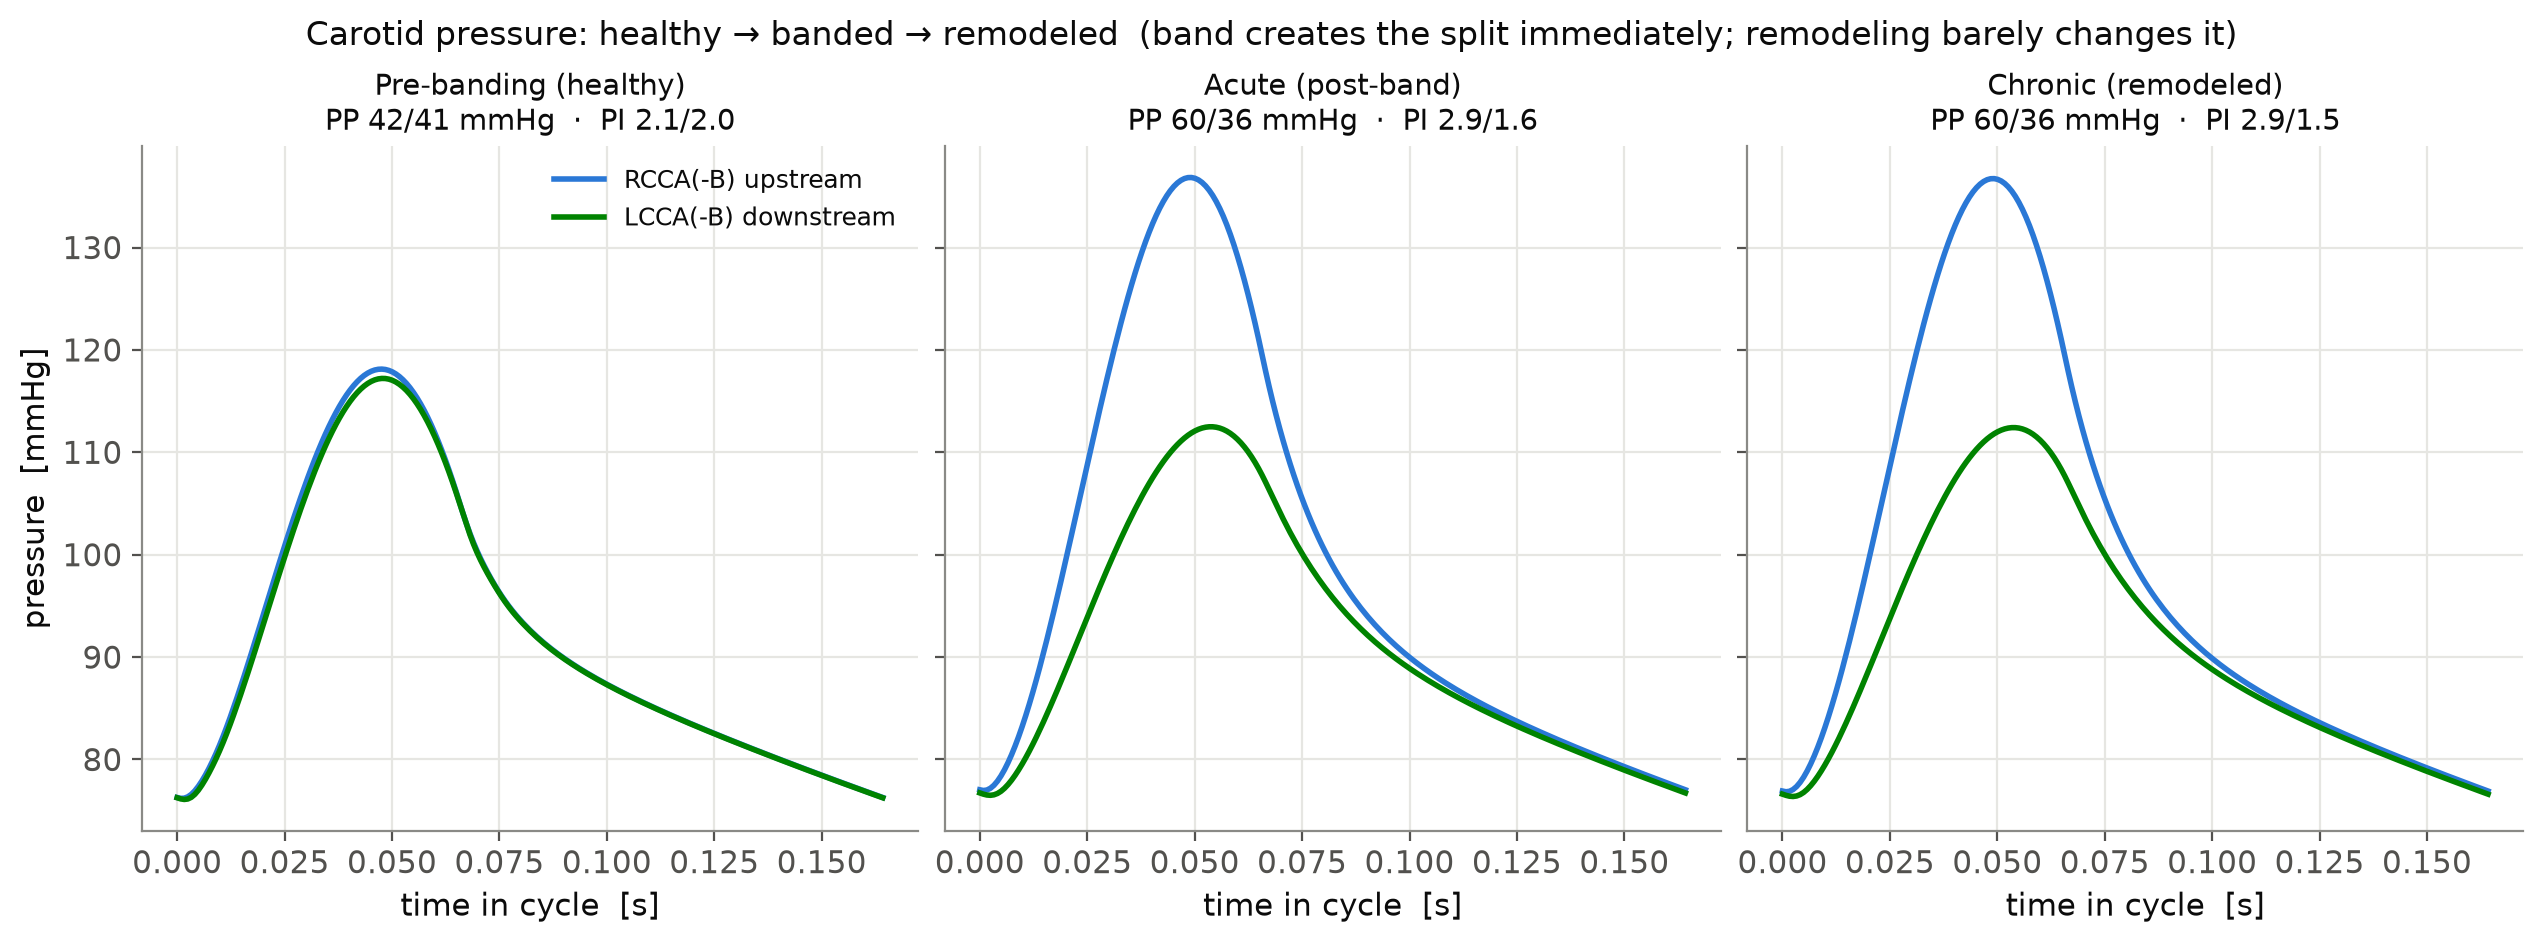
\includegraphics[height=0.62\textheight]{fig7_state_comparison.png}
\\[0.3em]
\footnotesize Carotid pressure is \textbf{symmetric before banding}, splits
\textbf{immediately} on banding (upstream $\uparrow$, downstream damped), and
\textbf{barely changes} with wall remodeling $\Rightarrow$ the split is set by
band \emph{position}; remodeling is the response, not the cause.
\end{frame}

% ---------------------------------------------------------------
\begin{frame}{Result: pulsatility vs.\ the paper}
\begin{columns}[c]
\begin{column}{0.55\textwidth}
\centering
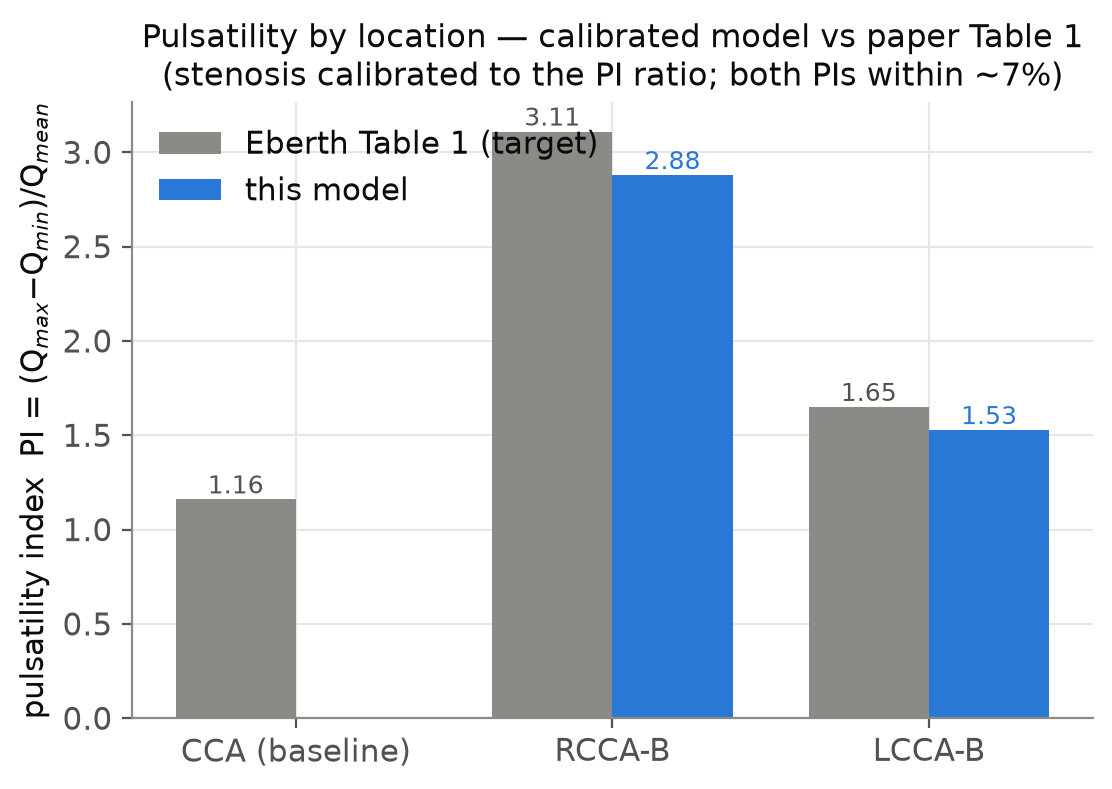
\includegraphics[width=\linewidth]{fig4_PI_validation.png}
\end{column}
\begin{column}{0.45\textwidth}
\small
\begin{tabular}{lcc}
\toprule
 & Paper & Model \\
\midrule
RCCA-B PI & 3.11 & $\approx 2.9$ \\
LCCA-B PI & 1.65 & $\approx 1.5$ \\
PI ratio  & 1.89 & 1.89 \\
PP RCCA-B & 56 & 60 \\
MAP (R/L) & similar & 98/91 \\
\bottomrule
\end{tabular}
\vspace{0.8em}

The \textbf{banded} carotids, the PI ratio, MAP similarity, and pulse pressure
are reproduced; mean carotid flows land in the measured range.
\end{column}
\end{columns}
\end{frame}

% ---------------------------------------------------------------
\begin{frame}{The band is a nonlinear (Young--Tsai) element}
\centering
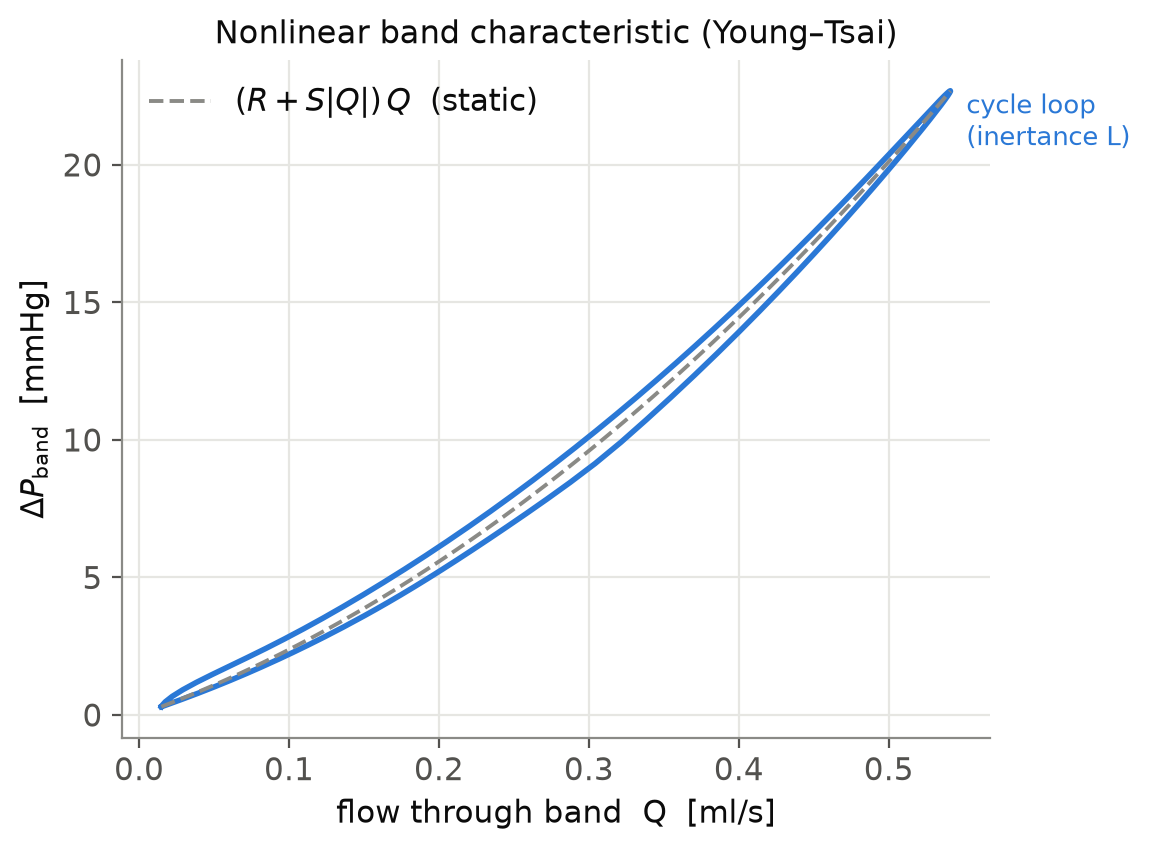
\includegraphics[height=0.62\textheight]{fig3_band_deltaP_Q.png}
\\[0.3em]
\footnotesize $\Delta P$--$Q$ across the band: the quadratic Bernoulli/turbulent
term ($S|Q|Q$) plus an inertance loop ($L\,\dot Q$). This nonlinearity + inertia
is what damps the downstream pulse while leaving the upstream node pulsatile.
\end{frame}

% ---------------------------------------------------------------
\begin{frame}{Limitation: baseline vs.\ banded cannot both be matched in 0D}
\begin{itemize}
  \item The model \textbf{over-predicts the baseline (pre-banding) PI}
        ($\approx 2.1$ vs.\ the paper's $1.16$), though baseline \emph{pulse
        pressure} matches ($\approx 41$ vs.\ $42$).
  \item A parameter sweep shows every knob that lowers the baseline PI to 1.16
        \alert{also collapses the banded PI} --- the passive bed is a linear
        pulsatility filter.
  \item The paper's baseline$\to$banded amplification is $\sim\!2.7\times$
        (1.16$\to$3.11); a lumped 0D band delivers only $\sim\!1.5\times$.
  \item The missing $\sim\!2\times$ is \textbf{wave reflection} off the band ---
        a spatial/timing effect a 0D element cannot represent.
\end{itemize}
\vspace{0.5em}
\centering\footnotesize
$\Rightarrow$ Reproducing the \emph{full} amplitude needs a \textbf{1D}
(wave-propagation) model --- exactly the 0D$\to$1D boundary.
\end{frame}

% ---------------------------------------------------------------
\begin{frame}{Summary}
\begin{itemize}
  \item A literature-parameterized 0D model reproduces the Eberth
        \textbf{pulsatility redistribution}: upstream carotid pulsatile,
        downstream damped, at matched mean pressure/flow.
  \item Banding creates the split \textbf{immediately}; wall remodeling barely
        changes it --- consistent with pulsatility being the \emph{stimulus}
        for remodeling.
  \item Quantitatively matches the \textbf{banded} carotids (PI ratio, MAP,
        pulse pressure); \textbf{over-predicts the baseline} --- a 0D
        limitation pointing to 1D wave reflection.
\end{itemize}
\end{frame}

\end{document}
